% Options for packages loaded elsewhere
\PassOptionsToPackage{unicode}{hyperref}
\PassOptionsToPackage{hyphens}{url}
%
\documentclass[
]{book}
\usepackage{amsmath,amssymb}
\usepackage{iftex}
\ifPDFTeX
  \usepackage[T1]{fontenc}
  \usepackage[utf8]{inputenc}
  \usepackage{textcomp} % provide euro and other symbols
\else % if luatex or xetex
  \usepackage{unicode-math} % this also loads fontspec
  \defaultfontfeatures{Scale=MatchLowercase}
  \defaultfontfeatures[\rmfamily]{Ligatures=TeX,Scale=1}
\fi
\usepackage{lmodern}
\ifPDFTeX\else
  % xetex/luatex font selection
\fi
% Use upquote if available, for straight quotes in verbatim environments
\IfFileExists{upquote.sty}{\usepackage{upquote}}{}
\IfFileExists{microtype.sty}{% use microtype if available
  \usepackage[]{microtype}
  \UseMicrotypeSet[protrusion]{basicmath} % disable protrusion for tt fonts
}{}
\makeatletter
\@ifundefined{KOMAClassName}{% if non-KOMA class
  \IfFileExists{parskip.sty}{%
    \usepackage{parskip}
  }{% else
    \setlength{\parindent}{0pt}
    \setlength{\parskip}{6pt plus 2pt minus 1pt}}
}{% if KOMA class
  \KOMAoptions{parskip=half}}
\makeatother
\usepackage{xcolor}
\usepackage{color}
\usepackage{fancyvrb}
\newcommand{\VerbBar}{|}
\newcommand{\VERB}{\Verb[commandchars=\\\{\}]}
\DefineVerbatimEnvironment{Highlighting}{Verbatim}{commandchars=\\\{\}}
% Add ',fontsize=\small' for more characters per line
\usepackage{framed}
\definecolor{shadecolor}{RGB}{248,248,248}
\newenvironment{Shaded}{\begin{snugshade}}{\end{snugshade}}
\newcommand{\AlertTok}[1]{\textcolor[rgb]{0.94,0.16,0.16}{#1}}
\newcommand{\AnnotationTok}[1]{\textcolor[rgb]{0.56,0.35,0.01}{\textbf{\textit{#1}}}}
\newcommand{\AttributeTok}[1]{\textcolor[rgb]{0.13,0.29,0.53}{#1}}
\newcommand{\BaseNTok}[1]{\textcolor[rgb]{0.00,0.00,0.81}{#1}}
\newcommand{\BuiltInTok}[1]{#1}
\newcommand{\CharTok}[1]{\textcolor[rgb]{0.31,0.60,0.02}{#1}}
\newcommand{\CommentTok}[1]{\textcolor[rgb]{0.56,0.35,0.01}{\textit{#1}}}
\newcommand{\CommentVarTok}[1]{\textcolor[rgb]{0.56,0.35,0.01}{\textbf{\textit{#1}}}}
\newcommand{\ConstantTok}[1]{\textcolor[rgb]{0.56,0.35,0.01}{#1}}
\newcommand{\ControlFlowTok}[1]{\textcolor[rgb]{0.13,0.29,0.53}{\textbf{#1}}}
\newcommand{\DataTypeTok}[1]{\textcolor[rgb]{0.13,0.29,0.53}{#1}}
\newcommand{\DecValTok}[1]{\textcolor[rgb]{0.00,0.00,0.81}{#1}}
\newcommand{\DocumentationTok}[1]{\textcolor[rgb]{0.56,0.35,0.01}{\textbf{\textit{#1}}}}
\newcommand{\ErrorTok}[1]{\textcolor[rgb]{0.64,0.00,0.00}{\textbf{#1}}}
\newcommand{\ExtensionTok}[1]{#1}
\newcommand{\FloatTok}[1]{\textcolor[rgb]{0.00,0.00,0.81}{#1}}
\newcommand{\FunctionTok}[1]{\textcolor[rgb]{0.13,0.29,0.53}{\textbf{#1}}}
\newcommand{\ImportTok}[1]{#1}
\newcommand{\InformationTok}[1]{\textcolor[rgb]{0.56,0.35,0.01}{\textbf{\textit{#1}}}}
\newcommand{\KeywordTok}[1]{\textcolor[rgb]{0.13,0.29,0.53}{\textbf{#1}}}
\newcommand{\NormalTok}[1]{#1}
\newcommand{\OperatorTok}[1]{\textcolor[rgb]{0.81,0.36,0.00}{\textbf{#1}}}
\newcommand{\OtherTok}[1]{\textcolor[rgb]{0.56,0.35,0.01}{#1}}
\newcommand{\PreprocessorTok}[1]{\textcolor[rgb]{0.56,0.35,0.01}{\textit{#1}}}
\newcommand{\RegionMarkerTok}[1]{#1}
\newcommand{\SpecialCharTok}[1]{\textcolor[rgb]{0.81,0.36,0.00}{\textbf{#1}}}
\newcommand{\SpecialStringTok}[1]{\textcolor[rgb]{0.31,0.60,0.02}{#1}}
\newcommand{\StringTok}[1]{\textcolor[rgb]{0.31,0.60,0.02}{#1}}
\newcommand{\VariableTok}[1]{\textcolor[rgb]{0.00,0.00,0.00}{#1}}
\newcommand{\VerbatimStringTok}[1]{\textcolor[rgb]{0.31,0.60,0.02}{#1}}
\newcommand{\WarningTok}[1]{\textcolor[rgb]{0.56,0.35,0.01}{\textbf{\textit{#1}}}}
\usepackage{longtable,booktabs,array}
\usepackage{calc} % for calculating minipage widths
% Correct order of tables after \paragraph or \subparagraph
\usepackage{etoolbox}
\makeatletter
\patchcmd\longtable{\par}{\if@noskipsec\mbox{}\fi\par}{}{}
\makeatother
% Allow footnotes in longtable head/foot
\IfFileExists{footnotehyper.sty}{\usepackage{footnotehyper}}{\usepackage{footnote}}
\makesavenoteenv{longtable}
\usepackage{graphicx}
\makeatletter
\def\maxwidth{\ifdim\Gin@nat@width>\linewidth\linewidth\else\Gin@nat@width\fi}
\def\maxheight{\ifdim\Gin@nat@height>\textheight\textheight\else\Gin@nat@height\fi}
\makeatother
% Scale images if necessary, so that they will not overflow the page
% margins by default, and it is still possible to overwrite the defaults
% using explicit options in \includegraphics[width, height, ...]{}
\setkeys{Gin}{width=\maxwidth,height=\maxheight,keepaspectratio}
% Set default figure placement to htbp
\makeatletter
\def\fps@figure{htbp}
\makeatother
\setlength{\emergencystretch}{3em} % prevent overfull lines
\providecommand{\tightlist}{%
  \setlength{\itemsep}{0pt}\setlength{\parskip}{0pt}}
\setcounter{secnumdepth}{5}
\usepackage{booktabs}
\ifLuaTeX
  \usepackage{selnolig}  % disable illegal ligatures
\fi
\usepackage[]{natbib}
\bibliographystyle{plainnat}
\IfFileExists{bookmark.sty}{\usepackage{bookmark}}{\usepackage{hyperref}}
\IfFileExists{xurl.sty}{\usepackage{xurl}}{} % add URL line breaks if available
\urlstyle{same}
\hypersetup{
  pdftitle={CFA Recovery},
  pdfauthor={JLB},
  hidelinks,
  pdfcreator={LaTeX via pandoc}}

\title{CFA Recovery}
\author{JLB}
\date{2024-08-26}

\begin{document}
\maketitle

{
\setcounter{tocdepth}{1}
\tableofcontents
}
\hypertarget{about}{%
\chapter*{About}\label{about}}
\addcontentsline{toc}{chapter}{About}

This bookdown project contains raw data, data analyses, and code to generate data visualizations for the paper \textbf{Inflammatory injury induces pain sensitization that is expressed beyond the site of injury in male (and not in female)}

\begin{itemize}
\item
  Raw data and code to generate the figure panels are available on our github.
\item
  Code to generate the figures and statistical analyses was written by Jennet Baumbach.
\item
  Any questions about these data should be directed to the corresponding author: Loren Martin, Ph.D \href{mailto:lj.martin@utoronto.ca}{\nolinkurl{lj.martin@utoronto.ca}}
\end{itemize}

\hypertarget{male-mice-homecage-behaviors-after-cfa}{%
\chapter{Male Mice: Homecage Behaviors after CFA}\label{male-mice-homecage-behaviors-after-cfa}}

\hypertarget{published-image}{%
\section*{Published Image}\label{published-image}}
\addcontentsline{toc}{section}{Published Image}

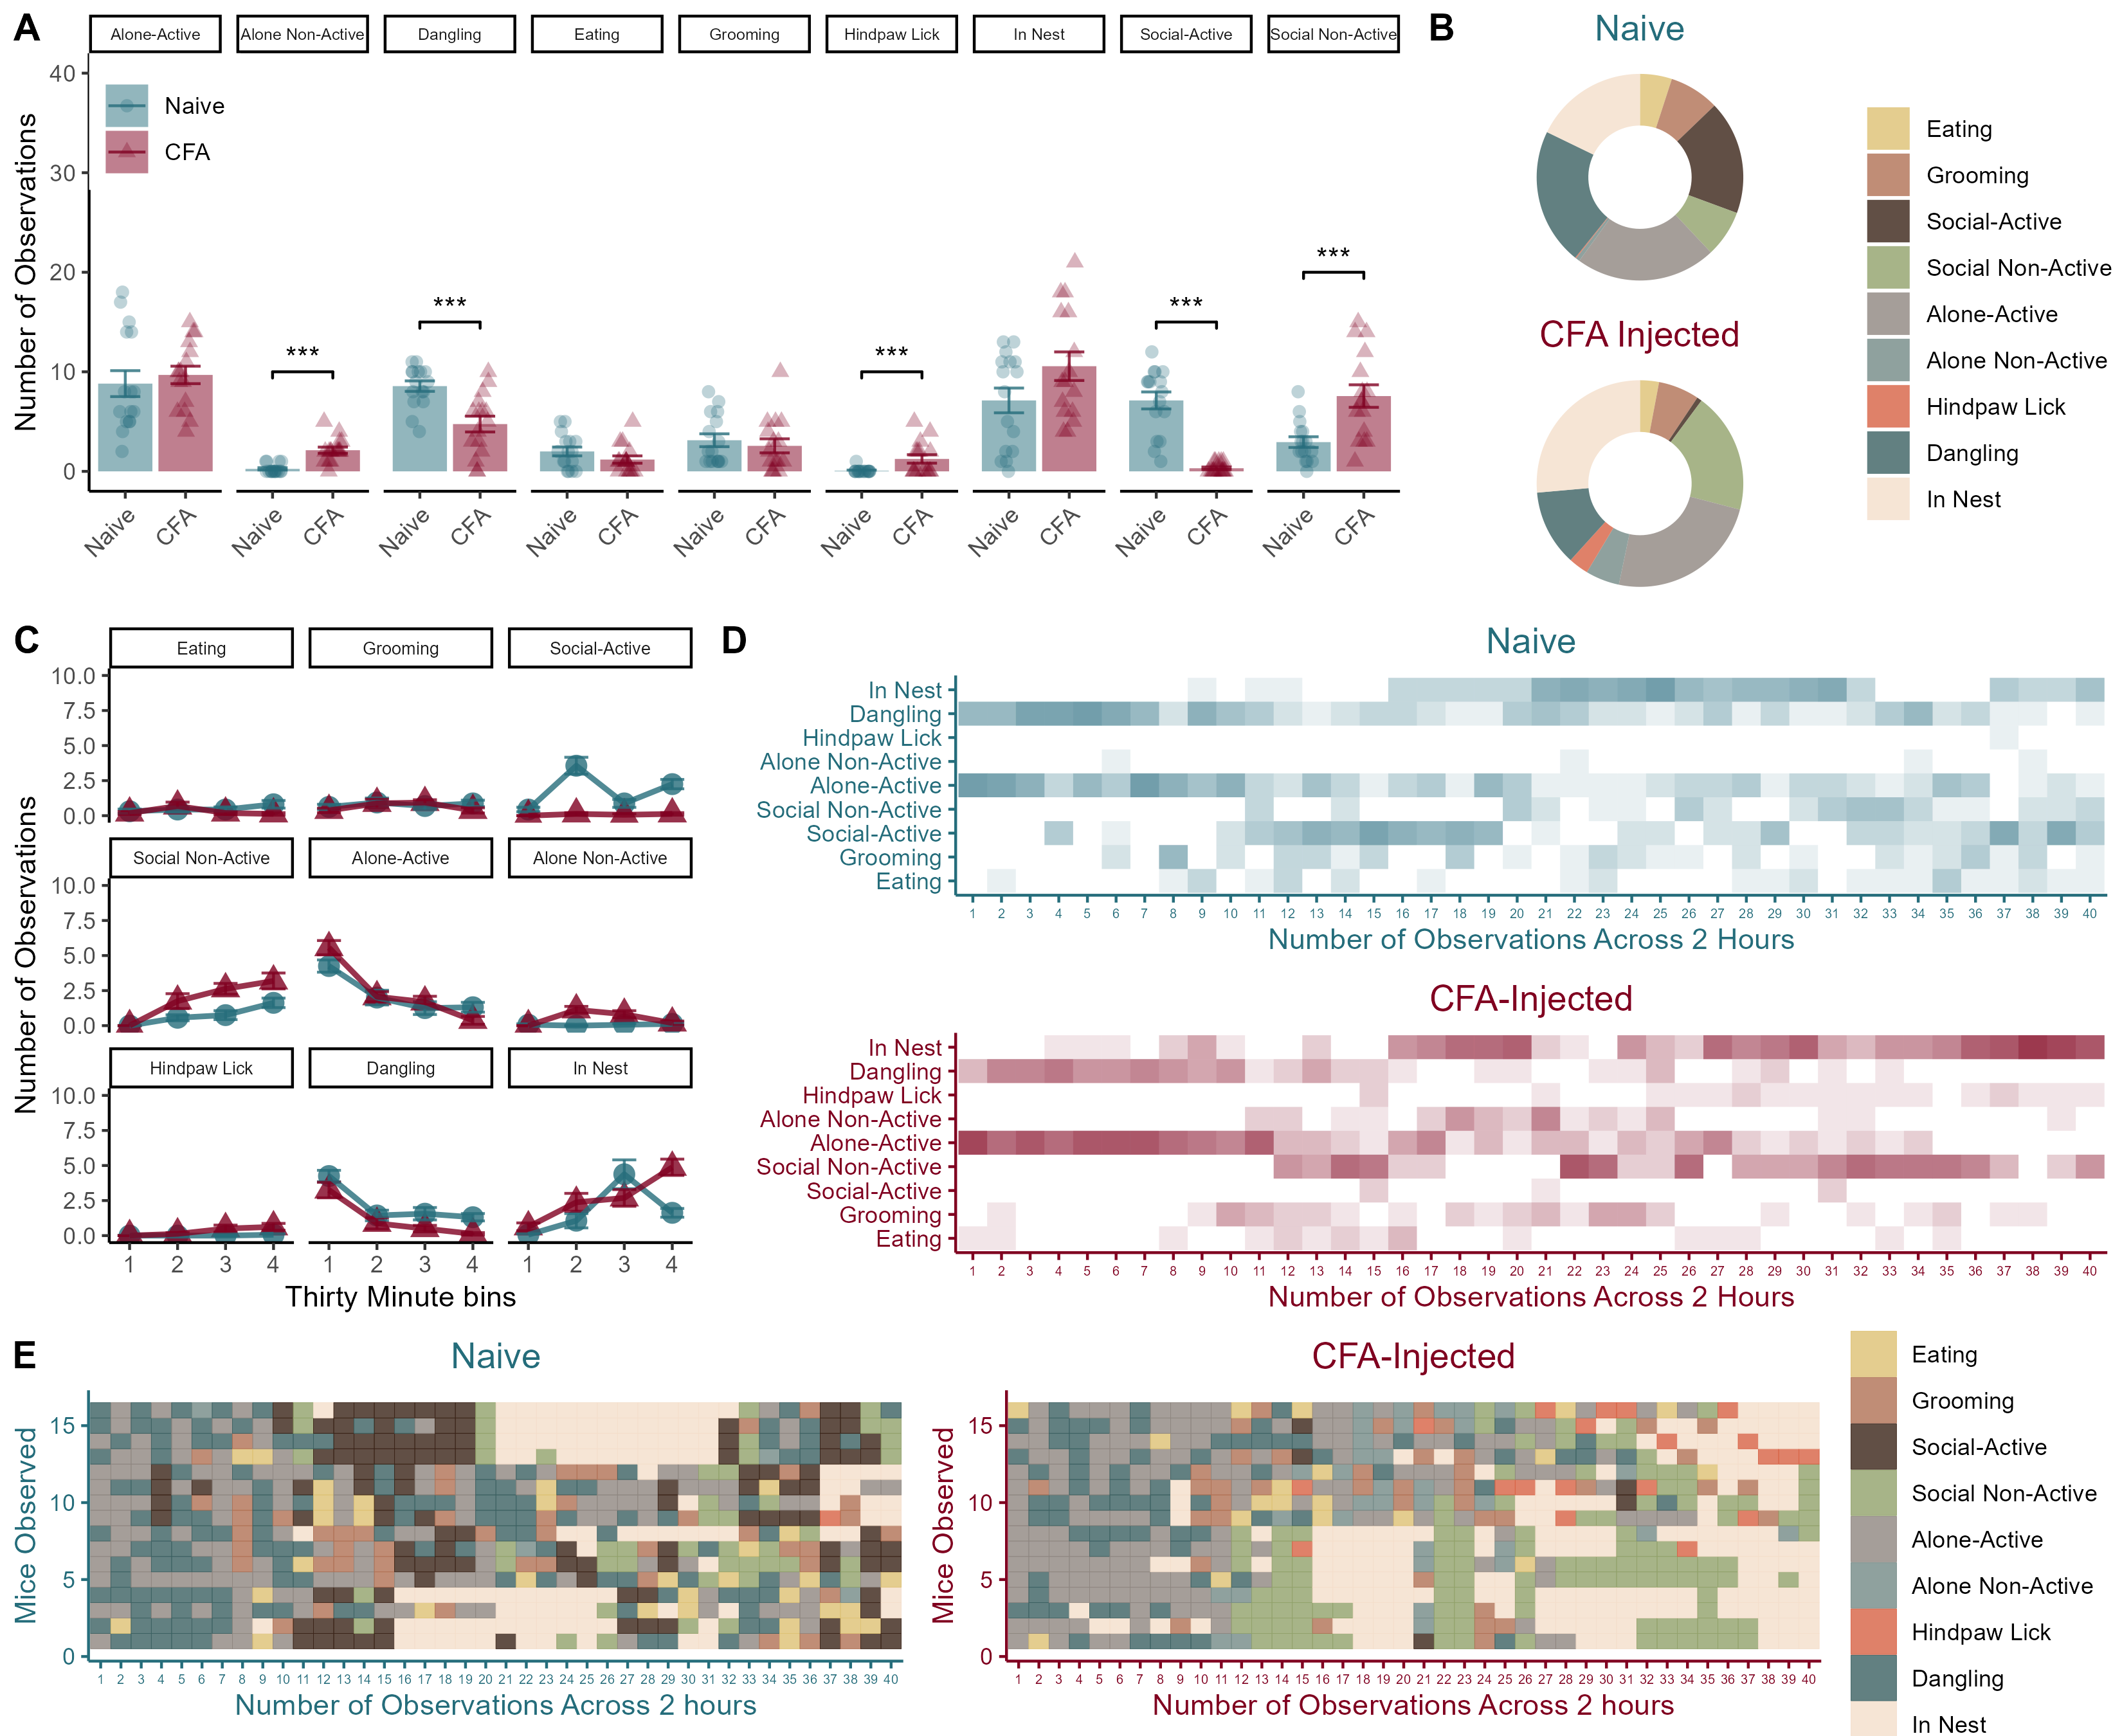
\includegraphics[width=45.83in]{Figs/1_male_HC_panel}

\textbf{Figure 1.} \emph{Homecage behaviors in male mice after an injection of 10}\(\mu l\) \emph{of 50\% CFA.} (A) Total number of observations of each behavior category across the two-hour observation period. (B) Donut charts showing the breakdown of average time spent engaging in each behavior for each group. (C) Line charts showcase group differences in changes in behavior across the two-hour long session. (D and E) are qualitative representations of the distribution of behaviors observed across the 40 time points. Data represented as mean value +/- SEM. *** indicates p \textless{} 0.001.

\hypertarget{statistical-analyses}{%
\section*{Statistical Analyses}\label{statistical-analyses}}
\addcontentsline{toc}{section}{Statistical Analyses}

\hypertarget{overall-manova-for-hc-behavs-for-males}{%
\subsection*{Overall MANOVA for HC Behavs for males}\label{overall-manova-for-hc-behavs-for-males}}
\addcontentsline{toc}{subsection}{Overall MANOVA for HC Behavs for males}

\begin{Shaded}
\begin{Highlighting}[]
\CommentTok{\# All behaviours in the model throws an error {-} it knows that you need to leave one out I suppose. }

\CommentTok{\# It is important to leave one behavior out of the MANOVA to allow for a degree of freedom in the analysis. }

\DocumentationTok{\#\# I thought originally that I would leave time in the nest out, but bc there is a clear sex difference in that behaviour I chose eating instead here: }

\NormalTok{fit }\OtherTok{\textless{}{-}} \FunctionTok{manova}\NormalTok{(}\FunctionTok{cbind}\NormalTok{(Grooming,}\StringTok{\textasciigrave{}}\AttributeTok{Social{-}Active}\StringTok{\textasciigrave{}}\NormalTok{,}\StringTok{\textasciigrave{}}\AttributeTok{Social Non{-}Active}\StringTok{\textasciigrave{}}\NormalTok{,}\StringTok{\textasciigrave{}}\AttributeTok{Alone{-}Active}\StringTok{\textasciigrave{}}\NormalTok{,}\StringTok{\textasciigrave{}}\AttributeTok{Alone Non{-}Active}\StringTok{\textasciigrave{}}\NormalTok{,}\StringTok{\textasciigrave{}}\AttributeTok{Hindpaw Lick}\StringTok{\textasciigrave{}}\NormalTok{,}\StringTok{\textasciigrave{}}\AttributeTok{Dangling}\StringTok{\textasciigrave{}}\NormalTok{,}\StringTok{\textasciigrave{}}\AttributeTok{In Nest}\StringTok{\textasciigrave{}}\NormalTok{) }\SpecialCharTok{\textasciitilde{}}\NormalTok{ Condition, }\AttributeTok{data=}\NormalTok{b)}
\FunctionTok{summary}\NormalTok{(fit)}
\end{Highlighting}
\end{Shaded}

\begin{verbatim}
##            Df Pillai approx F num Df den Df                Pr(>F)    
## Condition   1  0.536   17.183      8    119 < 0.00000000000000022 ***
## Residuals 126                                                        
## ---
## Signif. codes:  0 '***' 0.001 '**' 0.01 '*' 0.05 '.' 0.1 ' ' 1
\end{verbatim}

\begin{itemize}
\tightlist
\item
  The overall MANOVA for males was significant (F(1,30) = 43.46, p \textless{} 0.001), indicating that 10 \(\mu l\) of 50\% CFA altered patterns of behaviour during the two-hour interval after injection.
\end{itemize}

\hypertarget{follow-up-analyses}{%
\subsection*{Follow up analyses}\label{follow-up-analyses}}
\addcontentsline{toc}{subsection}{Follow up analyses}

\begin{Shaded}
\begin{Highlighting}[]
\CommentTok{\# Prints out the individual ANOVAs for each behaviour}
\FunctionTok{summary.aov}\NormalTok{(fit)}
\end{Highlighting}
\end{Shaded}

\begin{verbatim}
##  Response Grooming :
##              Df  Sum Sq Mean Sq F value Pr(>F)
## Condition     1   0.633 0.63281  0.7691 0.3822
## Residuals   126 103.672 0.82279               
## 
##  Response Social-Active :
##              Df Sum Sq Mean Sq F value           Pr(>F)    
## Condition     1  92.82  92.820   50.51 0.00000000007788 ***
## Residuals   126 231.55   1.838                             
## ---
## Signif. codes:  0 '***' 0.001 '**' 0.01 '*' 0.05 '.' 0.1 ' ' 1
## 
##  Response Social Non-Active :
##              Df Sum Sq Mean Sq F value    Pr(>F)    
## Condition     1  42.78  42.781  15.729 0.0001219 ***
## Residuals   126 342.72   2.720                      
## ---
## Signif. codes:  0 '***' 0.001 '**' 0.01 '*' 0.05 '.' 0.1 ' ' 1
## 
##  Response Alone-Active :
##              Df Sum Sq Mean Sq F value Pr(>F)
## Condition     1   1.53  1.5313  0.2959 0.5874
## Residuals   126 651.97  5.1744               
## 
##  Response Alone Non-Active :
##              Df Sum Sq Mean Sq F value     Pr(>F)    
## Condition     1  7.031  7.0312   17.83 0.00004588 ***
## Residuals   126 49.688  0.3943                       
## ---
## Signif. codes:  0 '***' 0.001 '**' 0.01 '*' 0.05 '.' 0.1 ' ' 1
## 
##  Response Hindpaw Lick :
##              Df Sum Sq Mean Sq F value   Pr(>F)   
## Condition     1  2.820 2.82031  10.231 0.001747 **
## Residuals   126 34.734 0.27567                    
## ---
## Signif. codes:  0 '***' 0.001 '**' 0.01 '*' 0.05 '.' 0.1 ' ' 1
## 
##  Response Dangling :
##              Df Sum Sq Mean Sq F value  Pr(>F)   
## Condition     1  29.07 29.0703  8.3725 0.00449 **
## Residuals   126 437.48  3.4721                   
## ---
## Signif. codes:  0 '***' 0.001 '**' 0.01 '*' 0.05 '.' 0.1 ' ' 1
## 
##  Response In Nest :
##              Df Sum Sq Mean Sq F value  Pr(>F)  
## Condition     1  23.63 23.6328   3.332 0.07031 .
## Residuals   126 893.67  7.0926                  
## ---
## Signif. codes:  0 '***' 0.001 '**' 0.01 '*' 0.05 '.' 0.1 ' ' 1
\end{verbatim}

\begin{itemize}
\tightlist
\item
  Male mice that were injected with CFA exhibited fewer socially-active behaviours (F(1,30) = 66.62, p \textless{} 0.001),
\item
  More socially inactive behaviours (F(1,30) = 14.55, p \textless{} 0.001),
\item
  More hindpaw licks (F(1,30) = 8.07, p = 0.008),
\item
  And less time dangling (F(1,30) = 17.19, p \textless{} 0.001).
\end{itemize}

\emph{Note} that the non-statistically significant results shown above are not reported in the mauscript.

\hypertarget{figure-2---female-mice-homecage-behaviors-after-cfa}{%
\chapter*{Figure 2 - Female Mice: Homecage Behaviors after CFA}\label{figure-2---female-mice-homecage-behaviors-after-cfa}}
\addcontentsline{toc}{chapter}{Figure 2 - Female Mice: Homecage Behaviors after CFA}

\hypertarget{published-image-1}{%
\section*{Published Image}\label{published-image-1}}
\addcontentsline{toc}{section}{Published Image}

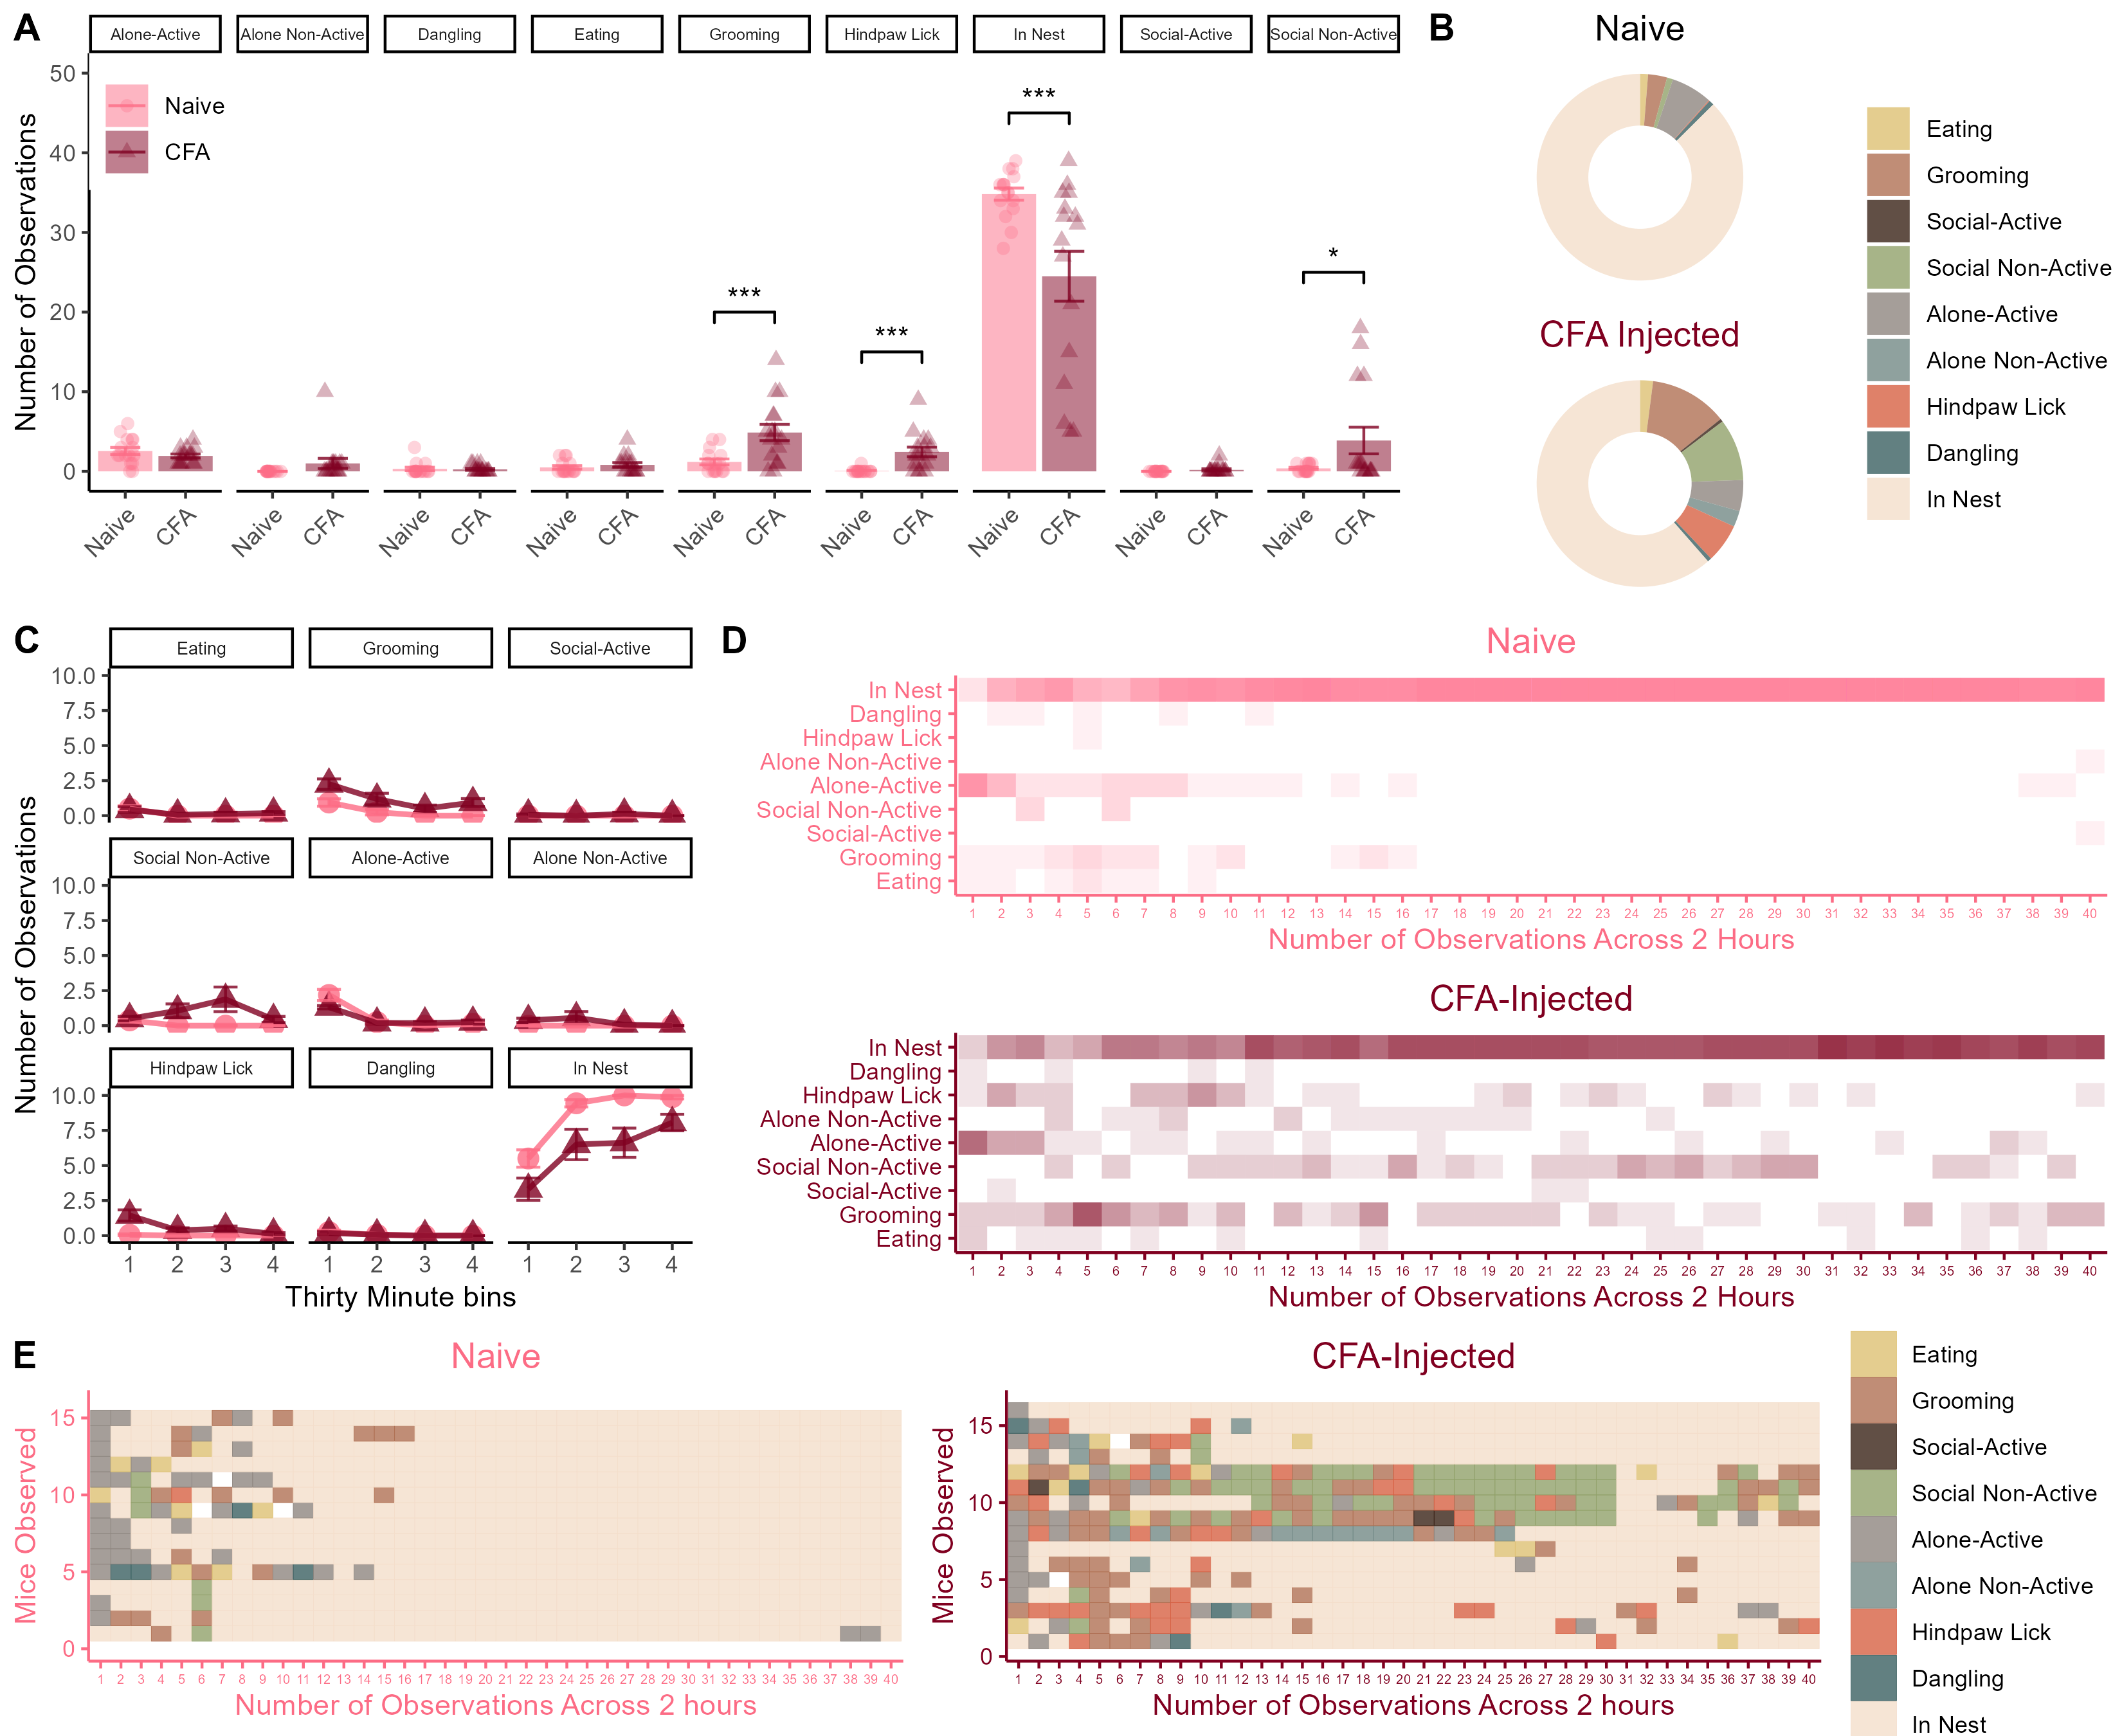
\includegraphics[width=45.83in]{Figs/2_female_HC_panel}

\textbf{Figure 2.} \emph{Homecage behaviors in female mice after injection of 10}\(\mu l\) \emph{of 50\% CFA.} (A) Total number of observations of each behavior category across the two-hour observation period. (B) Donut charts showing the breakdown of average time spent engaging in each behavior for each group. (C) Line charts showcase group differences in changes in behavior across the two-hour long session. (D and E) are qualitative representations of the distribution of behaviors observed across the 40 time points. Data represented as mean value +/- SEM. *** indicates p \textless{} 0.001.

\hypertarget{statistical-analyses-1}{%
\section*{Statistical Analyses}\label{statistical-analyses-1}}
\addcontentsline{toc}{section}{Statistical Analyses}

\hypertarget{overall-manova-for-hc-behavs-for-females}{%
\subsection{Overall MANOVA for HC Behavs for females}\label{overall-manova-for-hc-behavs-for-females}}

\begin{Shaded}
\begin{Highlighting}[]
\CommentTok{\# All behaviours in the model throws an error {-} it knows that you need to leave one out I suppose. }
\DocumentationTok{\#\# I thought originally that I would leave time in the nest out, but bc there is a clear sex difference in that behaviour I chose eating instead here: }

\NormalTok{fit }\OtherTok{\textless{}{-}} \FunctionTok{manova}\NormalTok{(}\FunctionTok{cbind}\NormalTok{(Grooming,}\StringTok{\textasciigrave{}}\AttributeTok{Social{-}Active}\StringTok{\textasciigrave{}}\NormalTok{,}\StringTok{\textasciigrave{}}\AttributeTok{Social Non{-}Active}\StringTok{\textasciigrave{}}\NormalTok{,}\StringTok{\textasciigrave{}}\AttributeTok{Alone{-}Active}\StringTok{\textasciigrave{}}\NormalTok{,}\StringTok{\textasciigrave{}}\AttributeTok{Alone Non{-}Active}\StringTok{\textasciigrave{}}\NormalTok{,}\StringTok{\textasciigrave{}}\AttributeTok{Hindpaw Lick}\StringTok{\textasciigrave{}}\NormalTok{,}\StringTok{\textasciigrave{}}\AttributeTok{Dangling}\StringTok{\textasciigrave{}}\NormalTok{,}\StringTok{\textasciigrave{}}\AttributeTok{In Nest}\StringTok{\textasciigrave{}}\NormalTok{) }\SpecialCharTok{\textasciitilde{}}\NormalTok{ Condition, }\AttributeTok{data=}\NormalTok{b)}
\FunctionTok{summary}\NormalTok{(fit)}
\end{Highlighting}
\end{Shaded}

\begin{verbatim}
##            Df Pillai approx F num Df den Df      Pr(>F)    
## Condition   1 0.2647    5.355      8    119 0.000009378 ***
## Residuals 126                                              
## ---
## Signif. codes:  0 '***' 0.001 '**' 0.01 '*' 0.05 '.' 0.1 ' ' 1
\end{verbatim}

\begin{itemize}
\tightlist
\item
  The overall MANOVA for female mice was also significant (F(1,30) = 3.05, p = 0.017)
\end{itemize}

\hypertarget{follow-up}{%
\subsection{Follow up:}\label{follow-up}}

\begin{Shaded}
\begin{Highlighting}[]
\CommentTok{\# Prints out the individual ANOVAs for each behaviour}
\FunctionTok{summary.aov}\NormalTok{(fit)}
\end{Highlighting}
\end{Shaded}

\begin{verbatim}
##  Response Grooming :
##              Df  Sum Sq Mean Sq F value     Pr(>F)    
## Condition     1  27.195 27.1953  20.121 0.00001617 ***
## Residuals   126 170.297  1.3516                       
## ---
## Signif. codes:  0 '***' 0.001 '**' 0.01 '*' 0.05 '.' 0.1 ' ' 1
## 
##  Response Social-Active :
##              Df Sum Sq  Mean Sq F value Pr(>F)
## Condition     1 0.0703 0.070313  1.8232 0.1794
## Residuals   126 4.8594 0.038566               
## 
##  Response Social Non-Active :
##              Df Sum Sq Mean Sq F value   Pr(>F)   
## Condition     1  24.50 24.5000  10.742 0.001354 **
## Residuals   126 287.38  2.2808                    
## ---
## Signif. codes:  0 '***' 0.001 '**' 0.01 '*' 0.05 '.' 0.1 ' ' 1
## 
##  Response Alone-Active :
##              Df  Sum Sq Mean Sq F value Pr(>F)
## Condition     1   0.781 0.78125  0.7768 0.3798
## Residuals   126 126.719 1.00570               
## 
##  Response Alone Non-Active :
##              Df Sum Sq Mean Sq F value  Pr(>F)  
## Condition     1      2 2.00000     4.5 0.03585 *
## Residuals   126     56 0.44444                  
## ---
## Signif. codes:  0 '***' 0.001 '**' 0.01 '*' 0.05 '.' 0.1 ' ' 1
## 
##  Response Hindpaw Lick :
##              Df Sum Sq Mean Sq F value     Pr(>F)    
## Condition     1 11.281 11.2813  19.682 0.00001971 ***
## Residuals   126 72.219  0.5732                       
## ---
## Signif. codes:  0 '***' 0.001 '**' 0.01 '*' 0.05 '.' 0.1 ' ' 1
## 
##  Response Dangling :
##              Df  Sum Sq  Mean Sq F value Pr(>F)
## Condition     1  0.0078 0.007813   0.095 0.7584
## Residuals   126 10.3594 0.082217               
## 
##  Response In Nest :
##              Df Sum Sq Mean Sq F value     Pr(>F)    
## Condition     1  212.7 212.695  20.546 0.00001336 ***
## Residuals   126 1304.4  10.352                       
## ---
## Signif. codes:  0 '***' 0.001 '**' 0.01 '*' 0.05 '.' 0.1 ' ' 1
\end{verbatim}

CFA-injected Female mice exhibited:

\begin{itemize}
\tightlist
\item
  Increased grooming during the observation session (F(1,30) = 12.26, p = 0.0015)
\item
  Increased social inactive behaviour (F(1,30) = 4.626, p = 0.039)
\item
  More hindpaw licks (F(1,30) = 15.95, p \textless{} 0.001)
\item
  And less observations in the nest (F(1,30) = 10.93, p = 0.002)
\end{itemize}

\begin{Shaded}
\begin{Highlighting}[]
\NormalTok{knitr}\SpecialCharTok{::}\NormalTok{opts\_chunk}\SpecialCharTok{$}\FunctionTok{set}\NormalTok{(}\AttributeTok{message =} \ConstantTok{FALSE}\NormalTok{, }
                      \AttributeTok{warning =} \ConstantTok{FALSE}\NormalTok{,}
                      \AttributeTok{echo =} \ConstantTok{FALSE}\NormalTok{,}
                      \AttributeTok{fig.align =} \StringTok{\textquotesingle{}center\textquotesingle{}}\NormalTok{)}
\FunctionTok{options}\NormalTok{(}\AttributeTok{scipen =} \DecValTok{999}\NormalTok{)}
\end{Highlighting}
\end{Shaded}

\hypertarget{figure-3---recovery-from-cfa-injury}{%
\chapter*{Figure 3 - Recovery from CFA Injury}\label{figure-3---recovery-from-cfa-injury}}
\addcontentsline{toc}{chapter}{Figure 3 - Recovery from CFA Injury}

\hypertarget{published-image-2}{%
\section*{Published Image}\label{published-image-2}}
\addcontentsline{toc}{section}{Published Image}

\begin{center}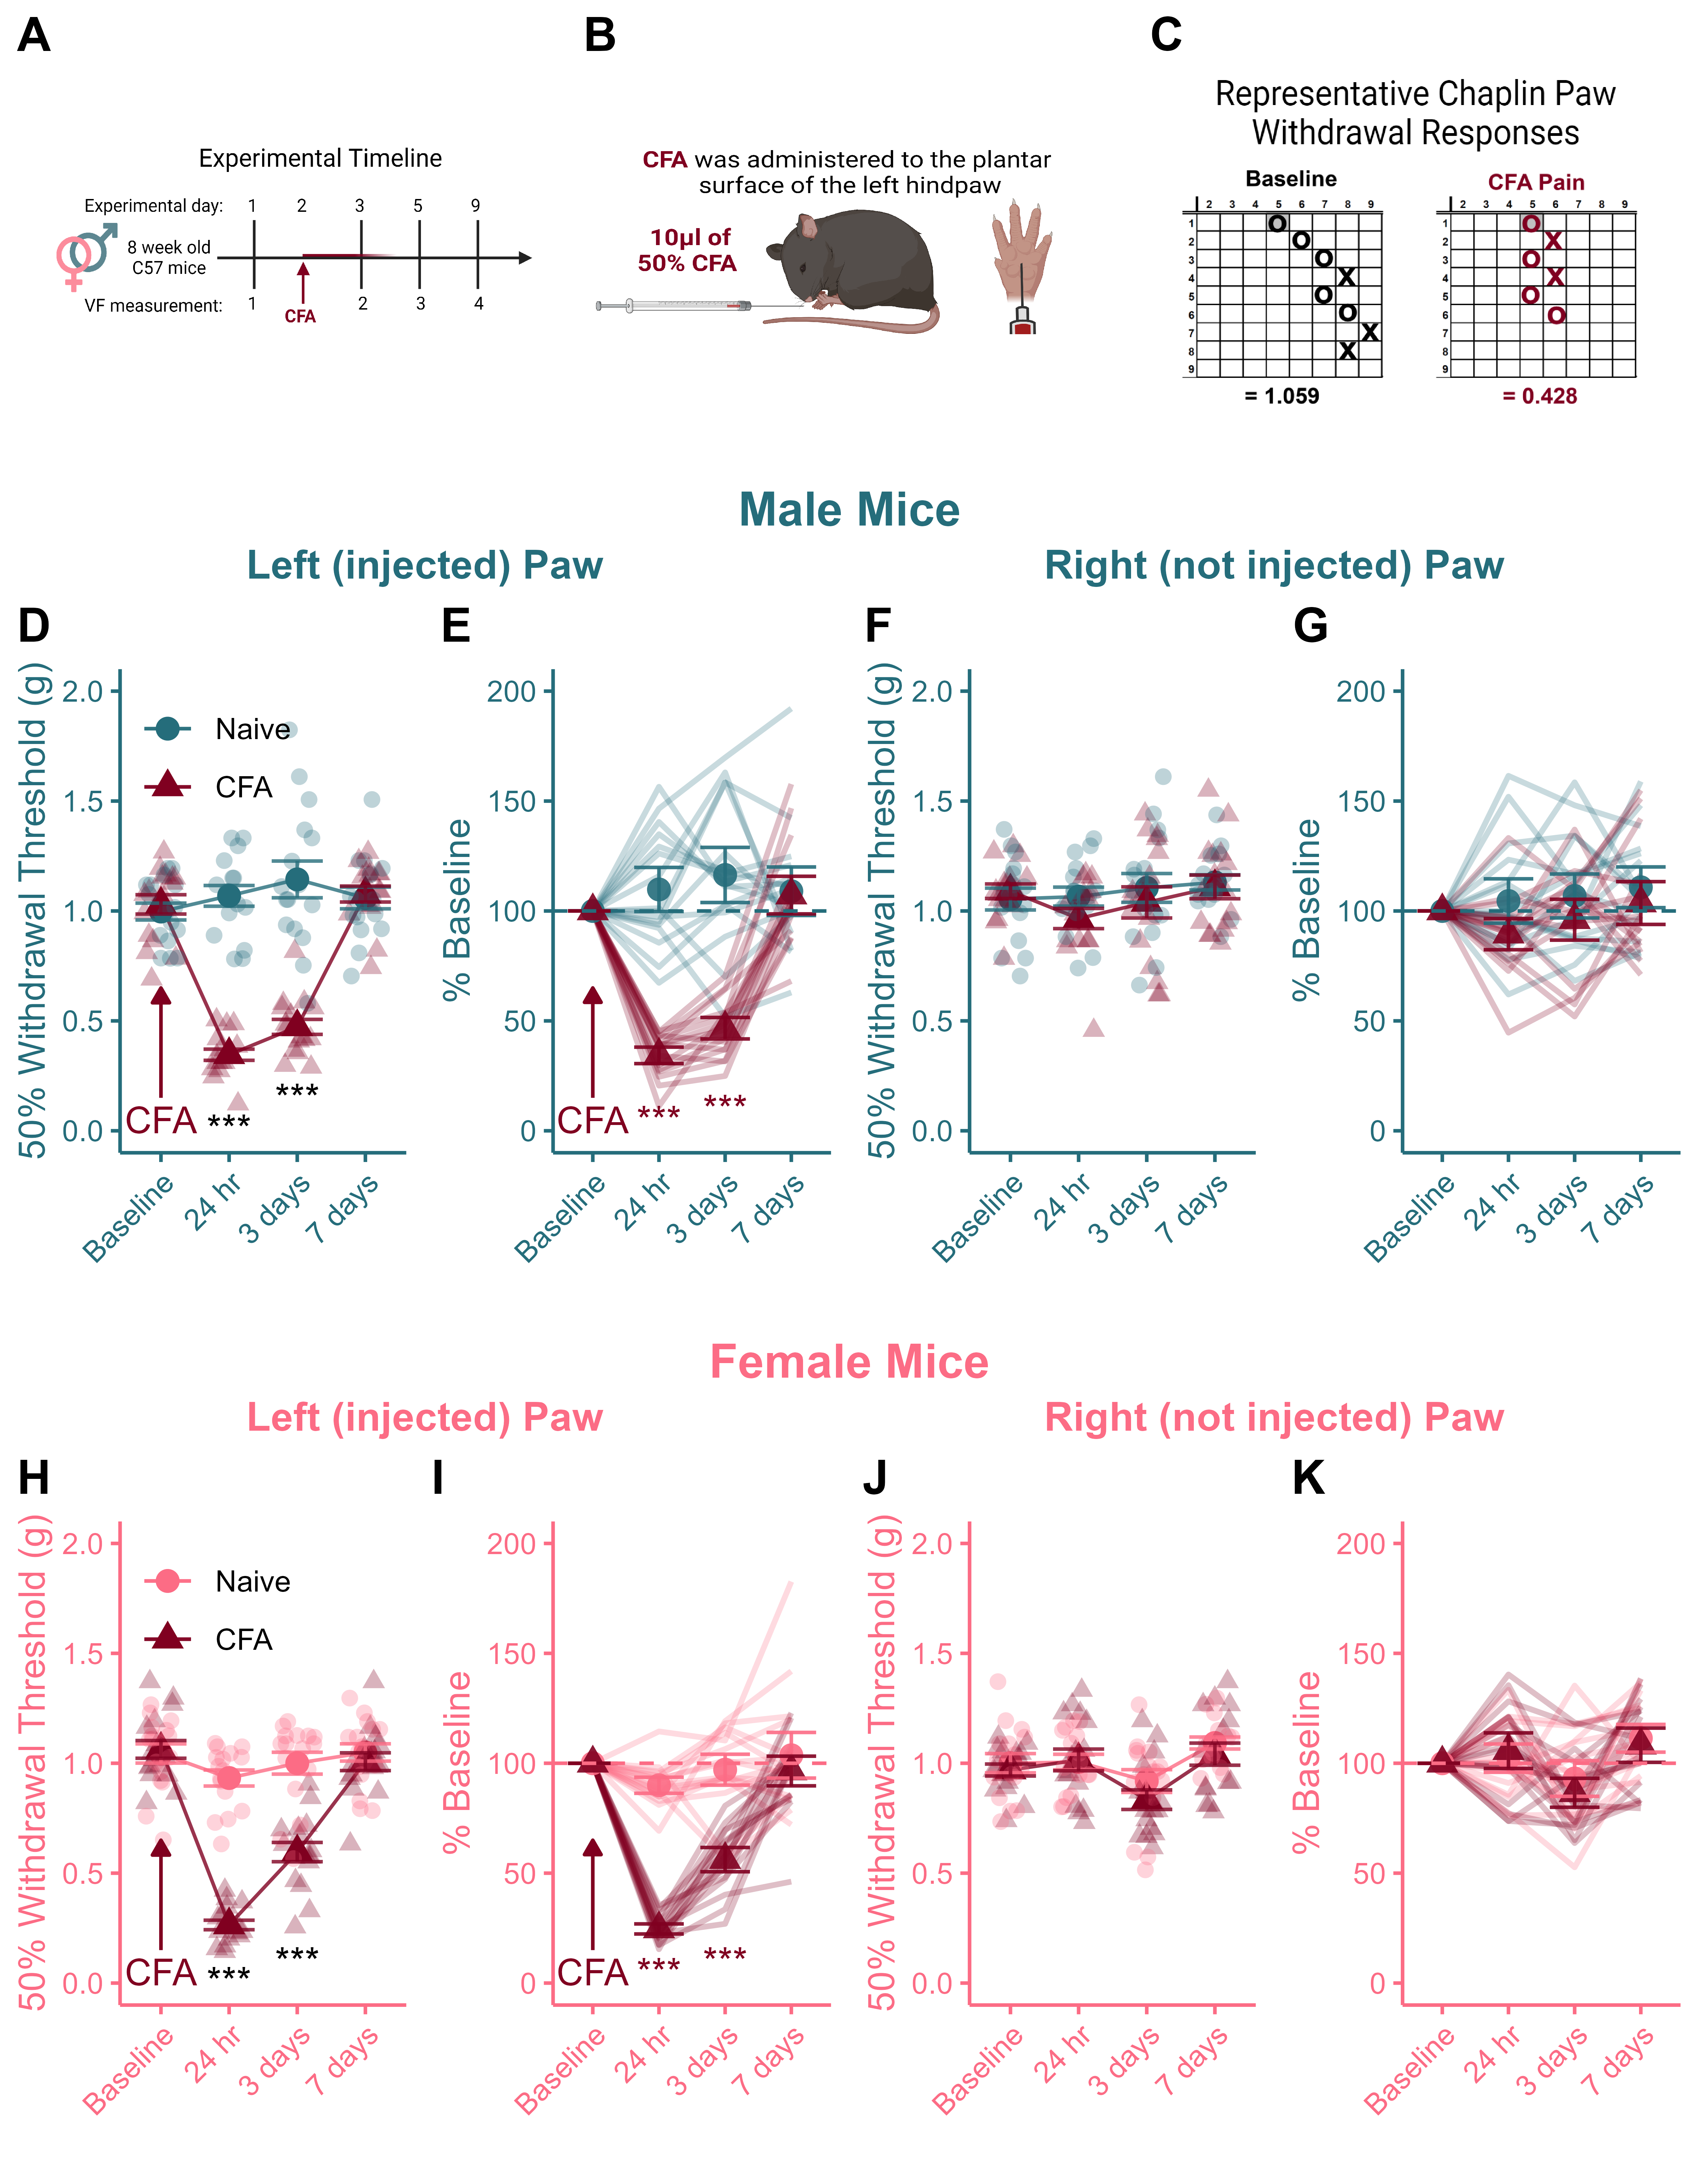
\includegraphics[width=68.06in]{Figs/3_VF_CFA_Recovery} \end{center}

\textbf{Figure 3.} \emph{CFA injection produces mechanical hypersensitivity that resolves within 7 days in male and female mice.} (A) Timeline of experimental testing. (B) Pain model to induce sensitization. (C) Representative images of Chaplan up-down von Frey measurements after CFA injection. CFA administration produces robust hypersensitivity at the site of injection that persists for at least 3 days and resolves within one week in both male (D, E) and female (H, I) mice. There were no changes in sensitivity of the contralateral (non-injected; right) hind paw during inflammatory pain and recovery from CFA injury in either males (F, G) or females (J, K). Data expressed as mean +/- SEM. *** Indicates between-group difference where \emph{p} \textless{} 0.001 and \# indicates a within-subject difference from baseline where \emph{p} \textless0.05.

\hypertarget{statistical-analyses-2}{%
\section*{Statistical Analyses}\label{statistical-analyses-2}}
\addcontentsline{toc}{section}{Statistical Analyses}

\begin{Shaded}
\begin{Highlighting}[]
\CommentTok{\# Select the left paws}
\NormalTok{left\_paws }\OtherTok{\textless{}{-}} \FunctionTok{rbind}\NormalTok{(female\_left,male\_left)}

\CommentTok{\# Switch to long form}
\NormalTok{a }\OtherTok{\textless{}{-}}\NormalTok{ left\_paws }\SpecialCharTok{\%\textgreater{}\%} 
  \FunctionTok{melt}\NormalTok{(}\AttributeTok{id.vars=}\FunctionTok{c}\NormalTok{(}\StringTok{"ID"}\NormalTok{,}\StringTok{"Sex"}\NormalTok{,}\StringTok{"CFA"}\NormalTok{))}

\CommentTok{\# Run RM anova on the 4 days of VF measuremenets}
\NormalTok{b }\OtherTok{\textless{}{-}} \FunctionTok{anova\_test}\NormalTok{(}\AttributeTok{data=}\NormalTok{a, }\AttributeTok{dv=}\NormalTok{value,}\AttributeTok{wid=}\NormalTok{ID,}\AttributeTok{between=}\FunctionTok{c}\NormalTok{(CFA,Sex),}\AttributeTok{within=}\NormalTok{variable,}\AttributeTok{effect.size=}\StringTok{"pes"}\NormalTok{)}
\NormalTok{knitr}\SpecialCharTok{::}\FunctionTok{kable}\NormalTok{(}\FunctionTok{get\_anova\_table}\NormalTok{(b))}
\end{Highlighting}
\end{Shaded}

\begin{tabular}{l|r|r|r|r|l|r}
\hline
Effect & DFn & DFd & F & p & p<.05 & pes\\
\hline
CFA & 1 & 60 & 128.271 & 0.000 & * & 0.681\\
\hline
Sex & 1 & 60 & 1.211 & 0.275 &  & 0.020\\
\hline
variable & 3 & 180 & 99.726 & 0.000 & * & 0.624\\
\hline
CFA:Sex & 1 & 60 & 1.314 & 0.256 &  & 0.021\\
\hline
CFA:variable & 3 & 180 & 91.678 & 0.000 & * & 0.604\\
\hline
Sex:variable & 3 & 180 & 2.651 & 0.050 &  & 0.042\\
\hline
CFA:Sex:variable & 3 & 180 & 3.570 & 0.015 & * & 0.056\\
\hline
\end{tabular}

\begin{itemize}
\item
  Significant main effects of CFA and timepoint.
\item
  Significant interaction between CFA and timepoint (F(3,180) = 91.67, p \textless{} 0.001)
\item
  Significant 3-way interaction between Sex, CFA and timepoint (F(3,180) = 3.57, p = 0.015)
\end{itemize}

\begin{Shaded}
\begin{Highlighting}[]
\CommentTok{\# Run two way ANOVAs for males and females separately: }

\DocumentationTok{\#\# Males}
\NormalTok{a }\SpecialCharTok{\%\textgreater{}\%}
  \FunctionTok{filter}\NormalTok{(Sex }\SpecialCharTok{==} \StringTok{"Male"}\NormalTok{) }\SpecialCharTok{\%\textgreater{}\%}
  \FunctionTok{anova\_test}\NormalTok{(}\AttributeTok{dv=}\NormalTok{value,}\AttributeTok{wid=}\NormalTok{ID,}\AttributeTok{between=}\NormalTok{CFA,}\AttributeTok{within=}\NormalTok{variable,}\AttributeTok{effect.size =} \StringTok{"pes"}\NormalTok{)}
\end{Highlighting}
\end{Shaded}

\begin{verbatim}
## ANOVA Table (type II tests)
## 
## $ANOVA
##         Effect DFn DFd      F                      p p<.05   pes
## 1          CFA   1  30 74.990 0.00000000117000000000     * 0.714
## 2     variable   3  90 31.478 0.00000000000005240000     * 0.512
## 3 CFA:variable   3  90 47.439 0.00000000000000000176     * 0.613
## 
## $`Mauchly's Test for Sphericity`
##         Effect     W     p p<.05
## 1     variable 0.897 0.681      
## 2 CFA:variable 0.897 0.681      
## 
## $`Sphericity Corrections`
##         Effect  GGe      DF[GG]                 p[GG] p[GG]<.05   HFe
## 1     variable 0.93 2.79, 83.67 0.0000000000003530000         * 1.035
## 2 CFA:variable 0.93 2.79, 83.67 0.0000000000000000242         * 1.035
##       DF[HF]                  p[HF] p[HF]<.05
## 1 3.1, 93.11 0.00000000000005240000         *
## 2 3.1, 93.11 0.00000000000000000176         *
\end{verbatim}

There is a significant interaction between CFA treatment and time point (F(3,90) = 47.44, p \textless{} 0.001)

\begin{verbatim}
## # A tibble: 4 x 10
##   variable .y.   group1 group2    n1    n2        p p.signif    p.adj
## * <fct>    <chr> <chr>  <chr>  <int> <int>    <dbl> <chr>       <dbl>
## 1 BL_L     value Naive  CFA       16    16 5.68e- 1 ns       5.68e- 1
## 2 hr_24    value Naive  CFA       16    16 1.22e-14 ****     1.22e-14
## 3 days_3   value Naive  CFA       16    16 1.46e- 8 ****     1.46e- 8
## 4 days_7   value Naive  CFA       16    16 7.67e- 1 ns       7.67e- 1
## # i 1 more variable: p.adj.signif <chr>
\end{verbatim}

\begin{itemize}
\item
  CFA-injected males have lower paw withdrawal thresholds than naive males 24 hours and 3 days post CFA administration (both p \textless{} 0.001).
\item
  There is no difference between the groups at baseline or 7 days post injection.
\end{itemize}

\begin{verbatim}
## ANOVA Table (type II tests)
## 
## $ANOVA
##         Effect DFn DFd      F                              p p<.05   pes
## 1          CFA   1  30 53.808 0.0000000359999999999999981061     * 0.642
## 2     variable   3  90 84.569 0.0000000000000000000000000427     * 0.738
## 3 CFA:variable   3  90 47.938 0.0000000000000000013200000000     * 0.615
## 
## $`Mauchly's Test for Sphericity`
##         Effect     W     p p<.05
## 1     variable 0.507 0.002     *
## 2 CFA:variable 0.507 0.002     *
## 
## $`Sphericity Corrections`
##         Effect   GGe      DF[GG]                    p[GG] p[GG]<.05   HFe
## 1     variable 0.754 2.26, 67.88 0.0000000000000000000289         * 0.819
## 2 CFA:variable 0.754 2.26, 67.88 0.0000000000000135000000         * 0.819
##       DF[HF]                      p[HF] p[HF]<.05
## 1 2.46, 73.7 0.000000000000000000000841         *
## 2 2.46, 73.7 0.000000000000001180000000         *
\end{verbatim}

\begin{itemize}
\tightlist
\item
  CFA-injected female mice also have lower paw withdrawal thresholds than naive males 24 hours and 3 days post CFA administration (both p \textless{} 0.001).
\end{itemize}

\begin{verbatim}
## # A tibble: 4 x 10
##   variable .y.   group1 group2    n1    n2        p p.signif    p.adj
## * <fct>    <chr> <chr>  <chr>  <int> <int>    <dbl> <chr>       <dbl>
## 1 BL_L     value Naive  CFA       16    16 7.49e- 1 ns       7.49e- 1
## 2 hr_24    value Naive  CFA       16    16 1.95e-16 ****     1.95e-16
## 3 days_3   value Naive  CFA       16    16 5.94e- 7 ****     5.94e- 7
## 4 days_7   value Naive  CFA       16    16 4.46e- 1 ns       4.46e- 1
## # i 1 more variable: p.adj.signif <chr>
\end{verbatim}

\begin{itemize}
\item
  CFA-injected males have lower paw withdrawal thresholds than naive males 24 hours and 3 days post CFA administration (both p \textless{} 0.001).
\item
  There is no difference between the groups at baseline or 7 days post injection.
\end{itemize}

\begin{verbatim}
## # A tibble: 8 x 11
##   Sex    variable .y.   group1 group2    n1    n2        p p.signif    p.adj
## * <chr>  <fct>    <chr> <chr>  <chr>  <int> <int>    <dbl> <chr>       <dbl>
## 1 Female BL_L     value Naive  CFA       16    16 7.49e- 1 ns       7.49e- 1
## 2 Female hr_24    value Naive  CFA       16    16 1.95e-16 ****     1.95e-16
## 3 Female days_3   value Naive  CFA       16    16 5.94e- 7 ****     5.94e- 7
## 4 Female days_7   value Naive  CFA       16    16 4.46e- 1 ns       4.46e- 1
## 5 Male   BL_L     value Naive  CFA       16    16 5.68e- 1 ns       5.68e- 1
## 6 Male   hr_24    value Naive  CFA       16    16 1.22e-14 ****     1.22e-14
## 7 Male   days_3   value Naive  CFA       16    16 1.46e- 8 ****     1.46e- 8
## 8 Male   days_7   value Naive  CFA       16    16 7.67e- 1 ns       7.67e- 1
## # i 1 more variable: p.adj.signif <chr>
\end{verbatim}

\begin{verbatim}
## # A tibble: 8 x 11
##   CFA   variable .y.   group1 group2    n1    n2      p p.signif  p.adj
## * <fct> <fct>    <chr> <chr>  <chr>  <int> <int>  <dbl> <chr>     <dbl>
## 1 Naive BL_L     value Female Male      16    16 0.408  ns       0.408 
## 2 Naive hr_24    value Female Male      16    16 0.0254 *        0.0254
## 3 Naive days_3   value Female Male      16    16 0.139  ns       0.139 
## 4 Naive days_7   value Female Male      16    16 0.871  ns       0.871 
## 5 CFA   BL_L     value Female Male      16    16 0.571  ns       0.571 
## 6 CFA   hr_24    value Female Male      16    16 0.017  *        0.017 
## 7 CFA   days_3   value Female Male      16    16 0.0288 *        0.0288
## 8 CFA   days_7   value Female Male      16    16 0.194  ns       0.194 
## # i 1 more variable: p.adj.signif <chr>
\end{verbatim}

\begin{itemize}
\item
  There was a sex difference in CFA-induced hypersensitivity both 24 hours (p = 0.017) and 3 days (p = 0.0288) post injection.
\item
  Female mice exhibited MORE sensitiivty than males at the 24hour time point, and LESS sensitivity than males 3-days after CFA.
\end{itemize}

\begin{verbatim}
## # A tibble: 24 x 11
##    Sex    CFA   .y.   group1 group2    n1    n2        p p.signif    p.adj
##  * <chr>  <fct> <chr> <chr>  <chr>  <int> <int>    <dbl> <chr>       <dbl>
##  1 Female Naive value BL_L   hr_24     16    16 6.03e- 2 ns       3.62e- 1
##  2 Female Naive value BL_L   days_3    16    16 4.52e- 1 ns       1   e+ 0
##  3 Female Naive value hr_24  days_3    16    16 2.52e- 1 ns       1   e+ 0
##  4 Female Naive value BL_L   days_7    16    16 9.36e- 1 ns       1   e+ 0
##  5 Female Naive value hr_24  days_7    16    16 5.06e- 2 ns       3.04e- 1
##  6 Female Naive value days_3 days_7    16    16 4.05e- 1 ns       1   e+ 0
##  7 Male   Naive value BL_L   hr_24     16    16 3.66e- 1 ns       1   e+ 0
##  8 Male   Naive value BL_L   days_3    16    16 6.7 e- 2 ns       4.02e- 1
##  9 Male   Naive value hr_24  days_3    16    16 3.43e- 1 ns       1   e+ 0
## 10 Male   Naive value BL_L   days_7    16    16 4.33e- 1 ns       1   e+ 0
## 11 Male   Naive value hr_24  days_7    16    16 9.04e- 1 ns       1   e+ 0
## 12 Male   Naive value days_3 days_7    16    16 2.86e- 1 ns       1   e+ 0
## 13 Female CFA   value BL_L   hr_24     16    16 1.10e-22 ****     6.59e-22
## 14 Female CFA   value BL_L   days_3    16    16 7.23e-13 ****     4.34e-12
## 15 Female CFA   value hr_24  days_3    16    16 2.18e- 8 ****     1.31e- 7
## 16 Female CFA   value BL_L   days_7    16    16 2.8 e- 1 ns       1   e+ 0
## 17 Female CFA   value hr_24  days_7    16    16 3.48e-21 ****     2.09e-20
## 18 Female CFA   value days_3 days_7    16    16 5.07e-11 ****     3.04e-10
## 19 Male   CFA   value BL_L   hr_24     16    16 1.25e-20 ****     7.5 e-20
## 20 Male   CFA   value BL_L   days_3    16    16 1.01e-16 ****     6.06e-16
## 21 Male   CFA   value hr_24  days_3    16    16 1.17e- 2 *        6.99e- 2
## 22 Male   CFA   value BL_L   days_7    16    16 3.38e- 1 ns       1   e+ 0
## 23 Male   CFA   value hr_24  days_7    16    16 5.52e-22 ****     3.31e-21
## 24 Male   CFA   value days_3 days_7    16    16 3.24e-18 ****     1.94e-17
## # i 1 more variable: p.adj.signif <chr>
\end{verbatim}

\begin{itemize}
\item
  CFA administration produced a robust hypersensitivity in the injected paw ( and not in the contralateral paw).
\item
  CFA-induced sensitivity resolved within one week post injection.
\end{itemize}

  \bibliography{book.bib,packages.bib}

\end{document}
